
\documentclass[11pt,titlepage,a4paper]{report}

%INCLUSIONE PACCHETTI
%---------------------------------------------
\usepackage[italian]{babel}
\usepackage{fancyhdr}
\usepackage{graphicx}
\graphicspath{{./pics/}}    % cartella di salvataggio immagini

% STILE DI PAGINA
%---------------------------------------------
\pagestyle{fancy}
\renewcommand{\sectionmark}[1]{\markright{\thesection.\ #1}}
\lhead{\nouppercase{\rightmark}}
\rhead{\nouppercase{\leftmark}}
\renewcommand{\chaptermark}[1]{%
\markboth{\thechapter.\ #1}{}}

%Ridefinisco lo stile plain della pagina
\fancypagestyle{plain}{%
	\lhead{
\includegraphics[height=50pt]{logo.eps}}
	\chead{}
	\rhead{HappyCode inc \\ happycodeinc@gmail.com}
	\lfoot{BR-jsys}
	\rfoot{\dt - \lv}
	\cfoot{\thepage}
	\renewcommand{\headrulewidth}{1pt}
	\renewcommand{\footrulewidth}{1pt}
}


\begin{document}


%definizione variabili 
\newcommand{\lv}{ 0.8 } % latest version
\newcommand{\dt}{ Specifica Tecnica }% Document title
\newcommand{\Glossario}{ Glossario.1.4.pdf }
\newcommand{\PdQ}{ PianoDiQualifica.1.1.pdf }
\newcommand{\PdP}{ PianoDiProgetto.1.1.pdf }

\newcommand{\br}{business rule}
\newcommand{\brs}{business rules}
\newcommand{\bo}{business object}
\newcommand{\bos}{business objects}
\newcommand{\re}{repository}
\newcommand{\brp}{BusinessRuleParser}
\newcommand{\brl}{BusinessRuleLexer}
\newcommand{\BR}{BusinessRule}

%fine definizione variabili


\hyphenation{glos-sa-rio es-pli-ci-to ve-ri-fi-ca-re re-po-si-to-ry se-gna-la-ta coe-ren-za}
\begin{titlepage}\begin{center}
\vspace*{0.5in}

\includegraphics{logo.eps}
\vspace*{0.2in} \\
{\Large \textbf{BR-jsys}}
{\Large \emph{business rules} per sistemi gestionali in architettura J2EE } 
\vspace{2in} \\
\Huge \textsc{ \dt }
\par\rule{10cm}{0.4pt} \par {\large Versione \lv - \today} \\
\end{center}\end{titlepage}
\vspace*{0.5in}


\begin{center}
\thispagestyle{plain}
\begin{table}[htbp]
\large{
\begin{tabular}{l}
\Large{\textbf{\textsf{Capitolato: ''BR-jsys``}}} \\
\begin{tabular}{||p{6cm}||p{6cm}||} \hline
\textbf{Data creazione:} & 18/11/2007 \\ \hline
\textbf{Versione:} & \lv \\ \hline
\textbf{Stato del documento:} & formale, esterno \\ \hline
% ----------------------------------------------------------------------------autori
\textbf{Redazione:} & Michele Bortolato \\ \hline
\textbf{Revisione:} & Alessia Trivellato, Elena Trivellato  \\ \hline
\textbf{Approvazione:}  & Mattia Meroi \\ \hline
\end{tabular} \\
\end{tabular}
}
\end{table}
\begin{table}[hbtp]
\large{
\begin{tabular}{l}
\Large{\textbf{\textsf{Lista di distribuzione}}} \\
\begin{tabular}{||p{6cm}||p{6cm}||} \hline
%  -------------------------------------------------------------lista di distribuzione
{HappyCode inc}& Gruppo di lavoro\\ \hline
{Tullio Vardanega, Renato Conte}& Rappresentanti del committente \\ \hline 
{Zucchetti S.r.l}& Azienda committente\\ \hline
\end{tabular} \\
\end{tabular}
}
\end{table}

\begin{table}[hbtp]
\large{
\begin{tabular}{l}
\Large{\textbf{\textsf{Diario delle modifiche}}} \\
\begin{tabular}{||p{2cm}||p{3.5cm}||p{6cm}||} \hline
%-------------------------------------------------------------------------------diario modifiche
\textbf{Versione} & \textbf{Data rilascio} & \textbf{Descrizione} \\ \hline
0.9 & 15/02/2008 & Correzione grammaticale \\ \hline
0.8 & 12/02/2008 & Modifiche ai diagrammi di attivit\`a e alle loro descrizioni\\ \hline
0.7 & 08/02/2008 & Aggiunta dei diagrammi di attivit\`a e rispettive descrizioni\\ \hline
0.6 & 06/02/2008 & Aggiunta dei diagrammi delle componenti e loro descrizione\\ \hline
0.5 & 05/02/2008 & Aggiunta del nome del file nel modello di documento\\ \hline
0.4 & 22/01/2008 & Modifica al layout dei documenti\\ \hline
0.3 & 22/12/2007 & Aggiornamento requisiti\\ \hline \hline
0.2 & 21/12/2007 & Documento sottoposto a revisionamento automatico\\ \hline
0.1 & 18/12/2007 & Stesura preliminare del documento \\ \hline

\end{tabular} \\
\end{tabular}

}
\end{table}
\end{center}
\newpage
\tableofcontents
\chapter{Introduzione}
\section{Scopo del documento}
Il presente documento descriver\`a il sistema software ``BR-jsys'' dal punto di vista architetturale e da noi implementato secondo le esigenze identificate nel documento ``Analisi dei Requisiti''. Attraverso l'uso di diagrammi UML, nella fattispecie con alcuni diagrammi delle classi, identificheremo alcune componenti principali nel quale scomporre il sistema. Procederemo inoltre con un approccio di tipo ``Bottom-up'' nelle procedure di verifica delle componenti. Questo documento fornir\`a quindi una visione pi\`u dettagliata delle componenti da realizzare; verr\`a definito il contesto d'uso del sistema e fornita la decomposizione di questo in componenti principali.
\section{Scopo del prodotto}
Per lo scopo del prodotto si faccia riferimento al documento ``Analisi dei Requisiti''.
\section{Glossario}
Viene fornito come documento esterno chiamato \Glossario .
\section{Riferimenti}
\begin{itemize}
\item Capitolato d'appalto concorso per sistema ``BR-jsys'';
\item ``Analisi dei Requisiti'';
\item ``Norme di Progetto'';
%\item \PdP
\item ``Piano di Qualifica'';
\item ``Piano di Progetto'';
%\item \PdQ
\item ``Ingegneria del software'' 8a edizione - Ian Sommerville;
\item ``The Definitive ANTLR Reference'';
\item Incontro con il committente ``Incontro2008-01-17.pdf'';
\item Incontro con il committente ``Incontro2008-02-05.pdf''.
\end{itemize}
%Ho tolto i riferimenti informativi

\chapter{Definizione del prodotto}
\subsection{Metodo e formalismo di specifica}
La progettazione del prodotto \`e stata attuata con l'uso di diagrammi UML 2.1, in quanto linguaggio internazionalmente riconosciuto e standardizzato.
Il software di cui l’azienda ha fatto uso per la creazione di quest'ultimi \`e \textit{Poseidon for UML Professional edition 6.0.2}. L'utilizzo di tale software deriva dalla completezza
di strumenti di cui \`e fornito, i quali soddisfano in pieno le nostre necessita'.

\subsection{Presentazione dell'architettura generale del sistema e identificazione dei componenti architetturali di alto livello}
Lo schema generale del prodotto \`e specificato nell'immagine sottostante.
\begin{center}
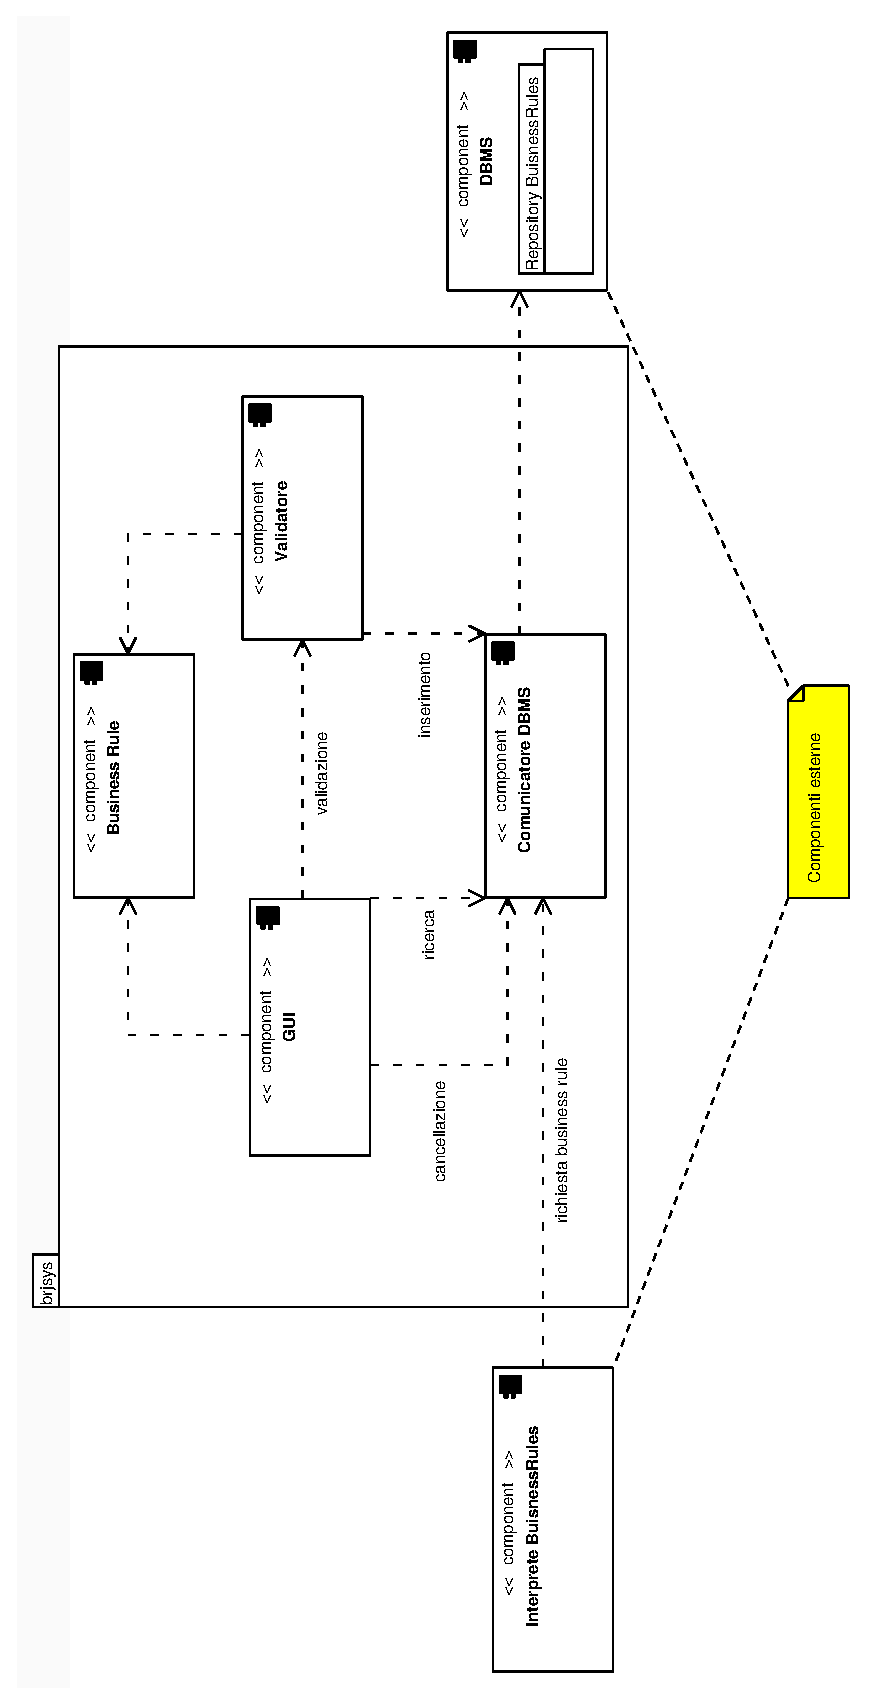
\includegraphics[width=0.8\textwidth, angle=-90]{DiagrammaClassi/schemagenerale.eps}
\end{center}
Abbiamo deciso di suddividere il prodotto in quattro macrocomponenti:
\begin{enumerate}
 \item \textbf{GUI}: Fornisce all'utente un interfaccia grafica minimale, consentendogli di effettuare operazioni di cancellazione e interrogazione del repository in maniera user-friendly.
\item \textbf{Business Rule}: Rappresenta la \br\ che l'utente dichiara e che deve essere passata al validatore per la compilazione.
\item \textbf{Validatore}: Accetta in input una \br, la valida e la inserisce se scritta correttamente nel \re.
\item \textbf{Comunicatore}: Si connette al DBMS esterno e comunica con esso tramite i formalismi del linguaggio XQuery.
Sar\`a appunto tramite Query che il DBMS effettuer\`a operazioni di inserimento, cancellazione o ricerca nel \re, qualora un componente lo richieda.
\end{enumerate}
Questa suddivisione, per quanto minimale, consente di individuare le componenti che verranno ampliamente descritte nel capitolo successivo.

\chapter{Descrizione dei singoli componenti}
Analizzeremo in seguito le quattro macrocomponenti elencate nel capitolo soprastante e ne daremo una descrizione pi\`u dettagliata.

\section{GUI}
\subsection{Diagramma delle classi}
\begin{center}
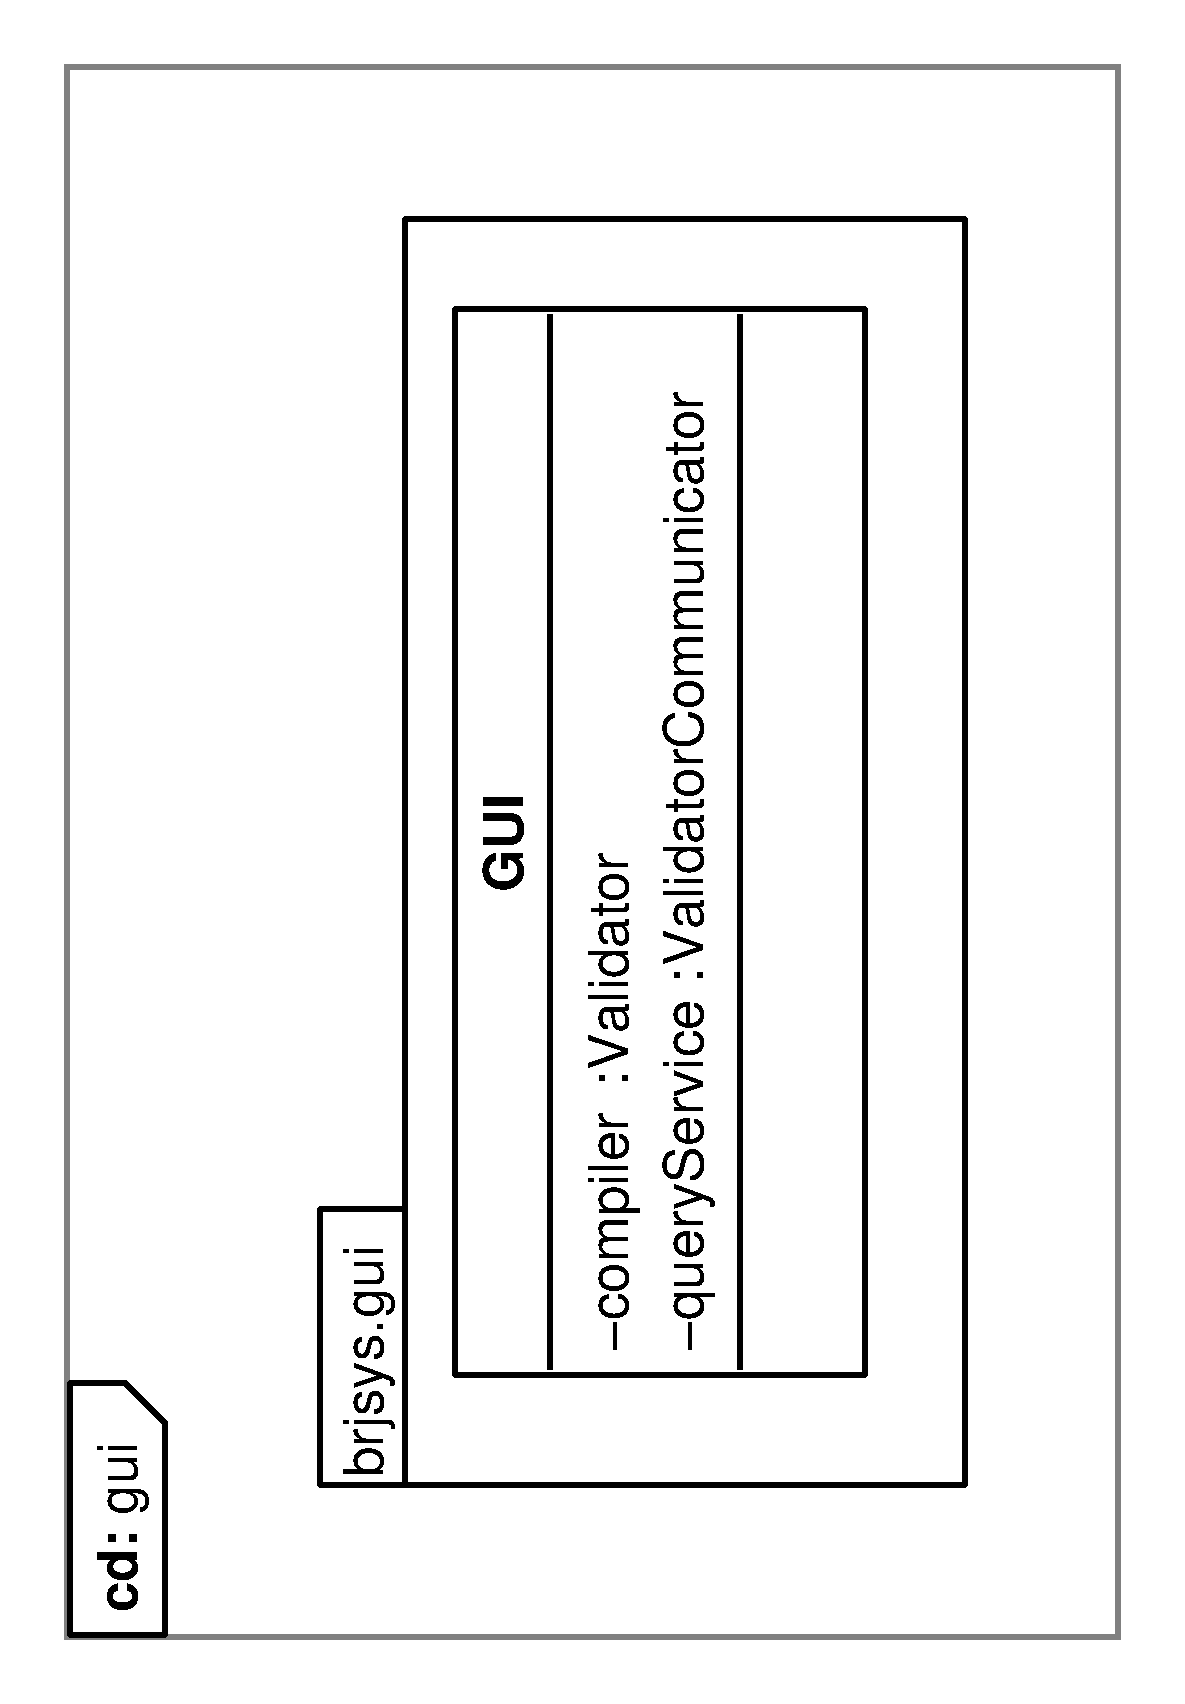
\includegraphics[width=0.3\textwidth, angle=-90]{DiagrammaClassi/gui.eps}
\end{center}
\subsection{Gui}
%Diagramma della classe GUI...comprensivo di package
\subsubsection{Tipo, obiettivo e funzione del componente}
Questa componente, realizzata tramite una singola classe java, fornisce all'utente un'interfaccia minimale che gli consente di effettuare operazioni di cancellazione e querying sul \re. Nel caso di esecuzione di una query definita dall'utente, verranno fornite anche informazioni relative ai tempi d'esecuzione.
\subsubsection{Relazioni d'uso di altre componenti}
Questa componente utilizza:
\begin{itemize}
 \item \BR\ per dichiarare una nuova \br\ da spedire al validatore;
 \item Validator per effettuare la validazione di una \br;
 \item GUICommunicator che tratteremo successivamente.
\end{itemize}
\subsubsection{Interfacce con e relazioni di uso da altre componenti}
Nessuna.
\subsubsection{Attivit\`a svolte e dati trattati}
Gui possiede i campi dato ``GUICommunicator'' e ``Validator'' che vengono utilizzati per fornire funzionalit\`a di interfacciamento che verranno trattate in seguito.

\section{Validatore}
\subsection{Diagramma delle classi}
\begin{center}
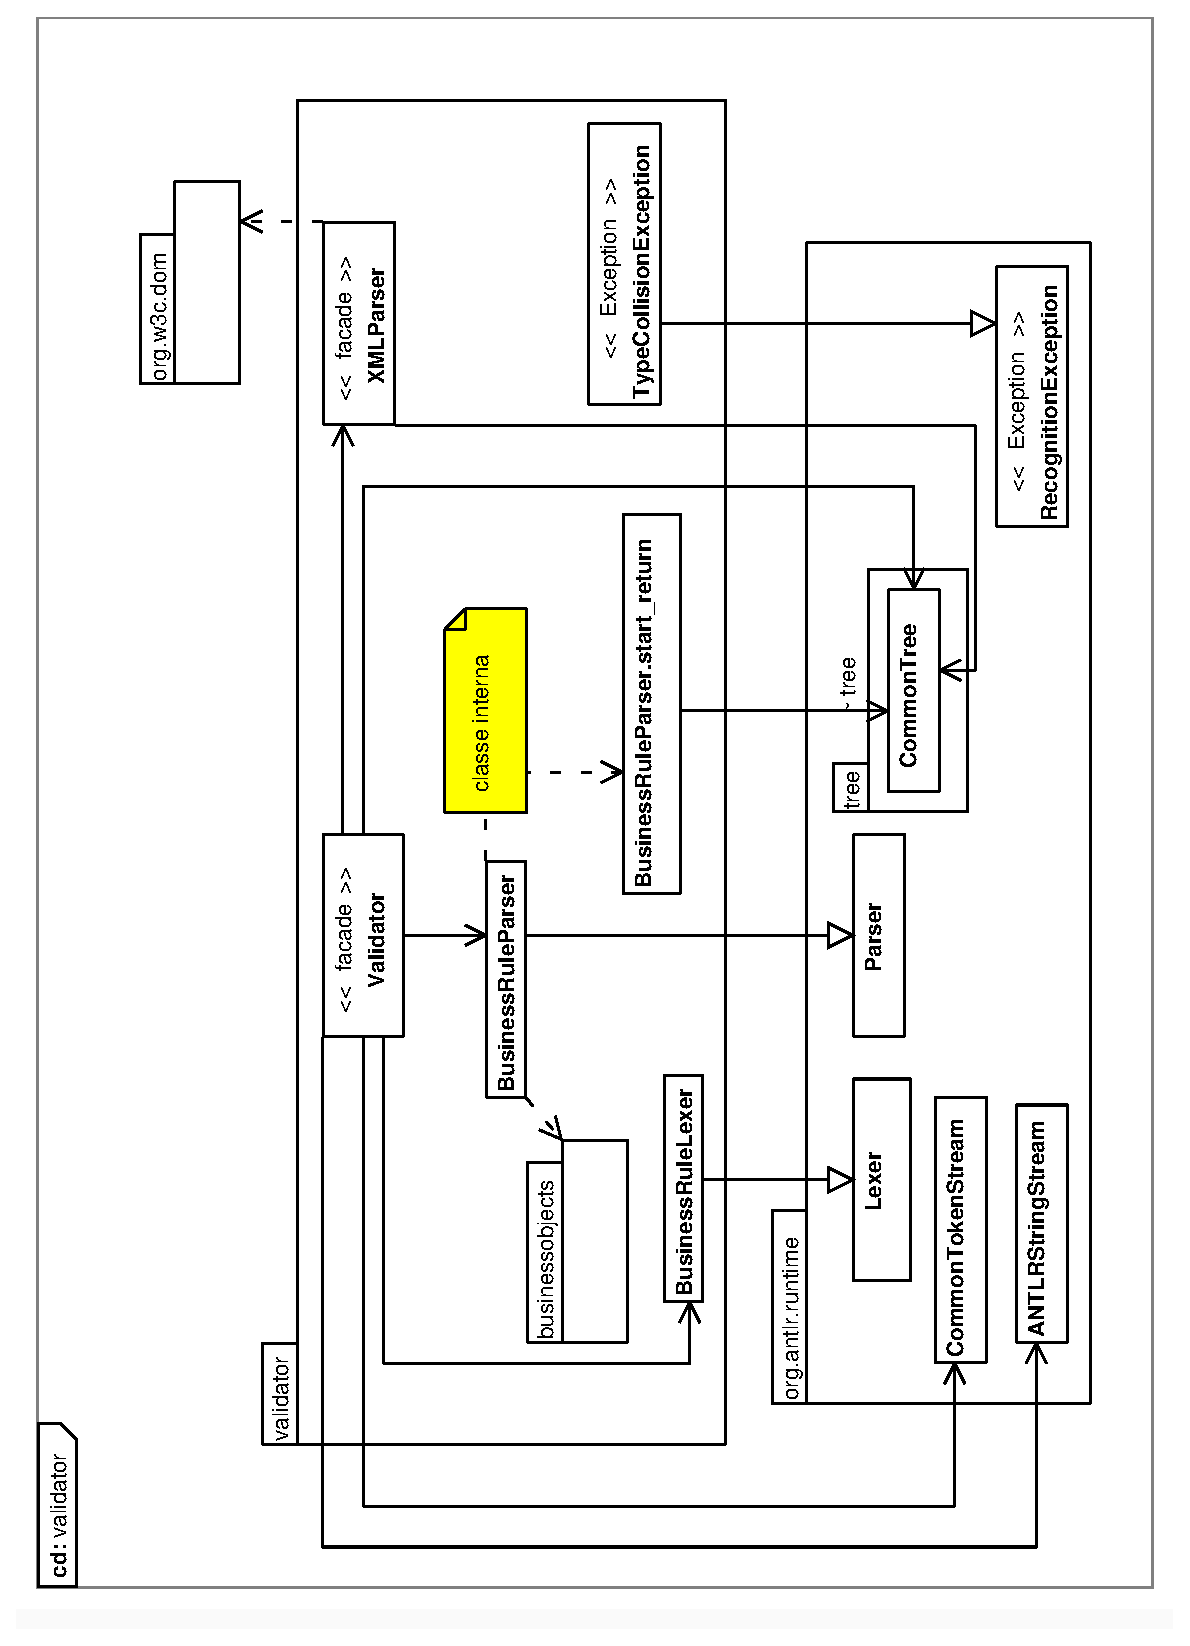
\includegraphics[width=0.6\textwidth, angle=-90]{DiagrammaClassi/validator.eps}
\end{center}
\subsection{Validator}%facade!!!->va descritto
\subsubsection{Tipo, obiettivo e funzione del componente}
Questa componente effettua la validazione di una \br, dando la possibilit\`a all'utilizzatore di evitare le singole operazioni di compilazione. Ha il ruolo di \textit{fa\c{c}ade}: fornisce un'interfaccia unificata che riesce a gestire in maniera semplice ed immediata le operazioni di compilazione e inserimento che avremmo altrimenti dovuto riportare direttamente dove la componente GUI lo richiedesse.
\subsubsection{Relazioni d'uso di altre componenti}
Validator usa le componenti \brp, \brl, XMLParser e ValidatorCommunicator. Quest'ultime verranno ampliamente descritte in seguito.
\subsubsection{Interfacce con e relazioni di uso da altre componenti}
Validator \`e in relazione con la componente GUI, al fine di rendere possibile la validazione.
\subsubsection{Attivit\`a svolte e dati trattati}
La componente contiene soltanto il metodo validate() che effettua la validazione della \br.

\subsection{BusinessRuleLexer}
\subsubsection{Tipo, obiettivo e funzione del componente}
Questa componente, derivata da org.antlr.runtime.Lexer, non \`e altro che una classe wrapper per la stringa che rappresenta la \br. Essa aggiunge funzionalit\`a alla stringa, necessarie per il successivo parsing.
\subsubsection{Relazioni d'uso di altre componenti}
Nessuna.
\subsubsection{Interfacce con e relazioni di uso da altre componenti}
La componente BusinessRuleParser necessita della componente BusinessRuleLexer. Quest'ultima verr\`a approfondita successivamente.
\subsubsection{Attivit\`a svolte e dati trattati}
BusinessRuleLexer mette a disposizione vari metodi per la lettura del testo della \br, nonch\`e per la gestione di eventuali eccezioni avvenute in fase di validazione.\\
\textit{\textbf{Nota:}Questa classe \`e stata creata utilizzando uno strumento automatico per la generazione di parser, data in input la specifica di una grammatica.}

\subsection{BusinessRuleParser}
\subsubsection{Tipo, obiettivo e funzione del componente}
Questa componente, derivata da org.antlr.runtime.Parser, effettua il parsing della stringa che rappresenta la \br. Effettua quindi il controllo sintattico della regola e il controllo semantico facendo un controllo sui tipi dei dati (siano essi costanti oppure campi dati di \bos). Mentre effettua la validazione BusinessRuleParser genera l'albero di parsing secondo le specifiche presenti nel controllo semantico. \`E in grado infine di dare informazioni accurate riguardo eventuali errori in fase di validazione.
\subsubsection{Relazioni d'uso di altre componenti}
Questa componente necessita di un TokenStream, fornitogli indirettamente da BusinessRuleLexer. Deve riferirsi poi alla componente BusinessObjects, per effettuare il controllo sui tipi per il \bo\ associato. Per trattare gli errori in fase di validazione, ha bisogno della componente TypeCollisionException.
\subsubsection{Interfacce con e relazioni di uso da altre componenti}
\brp\ viene messa in relazione con XMLParser che verr\`a trattata successivamente.
\`E utilizzata inoltre dalla componente Validator.
\subsubsection{Attivit\`a svolte e dati trattati}
\brp\ mette a disposizione vari metodi per effettuare il parsing e i test semantici. Dispone inoltre di numerosi campi dato per la ricognizione dei token.\\
\textit{\textbf{Nota:}Questa classe \`e stata creata utilizzando uno strumento automatico per la generazione di parser, data in input la specifica di una grammatica.}

\subsection{TypeCollisionException}
\subsubsection{Tipo, obiettivo e funzione del componente}
Questa componente, derivata dalla classe org.antlr.runtime.RecognitionException, permette di ricavare informazioni sugli eventuali errori avvenuti in fase di parsing della \br. In definitiva aggiunge alla sua superclasse la possibilit\`a di riportare informazioni su errori di tipo.
\subsubsection{Relazioni d'uso di altre componenti}
Nessuna.
\subsubsection{Interfacce con e relazioni di uso da altre componenti}
La componente TypeCollisionException \`e utilizzata da \brp\ per sollevare eccezioni derivanti da errori di tipo.
\subsubsection{Attivit\`a svolte e dati trattati}
Viene ridefinito il metodo printStackTrace() e messo a disposizione un costruttore per avere informazioni sui tipi che si sono rivelati incompatibili.

\subsection{XMLParser}%probabilmente è un facade anche questo
\subsubsection{Tipo, obiettivo e funzione del componente}
La componente XMLParser si occupa di effettuare la conversione dell'albero sintattico prodotto dalla componente \brp in un elemento XML rappresentante la \br. L'elemento XML risultante conterr\`a:
\begin{itemize}
 \item il nome della \br, che dovr\`a essere univoco;
 \item il nome del \bo\ associato alla regola;
 \item la struttura dell'AST della \br, scritta secondo la metodologia elemento-attributo tipica di XML;
 \item la struttura dell'AST della \br, scritta linearmente secondo la notazione prefissa rappresentata da un singolo attributo XML;
 \item la \br\ effettivamente digitata dall'utente;
 \item eventuali commenti associati dall'utente alla \br.
\end{itemize}
XMLParser ha in questo contesto il ruolo del design pattern \textit{fa\c{c}ade}; la creazione di un elemento XML tramite il package java \textit{org.w3c.dom} necessita di operazioni sequenziali che coinvolgono numerose classi e numerosi metodi. Implementare tutte queste procedure direttamente nella classe Validator renderebbe il codice meno leggibile e meno manipolabile.
\subsubsection{Relazioni d'uso di altre componenti}
XMLParser ha bisogno dell'AST prodotto da \brp, nonch\`e necessita della componente \br\ per ricavare le informazioni da inserire nell'elemento XML.
\subsubsection{Interfacce con e relazioni di uso da altre componenti}
La componente ValidatorCommunicator ha bisogno dell'elemento XML prodotto da XMLParser per avviare la procedura di inserimento nel \re.
\subsubsection{Attivit\`a svolte e dati trattati}
XMLParser  contiene le operazioni per scorrere l'AST ed effettuare la traduzione in XML.Inoltre dispone di una tabella Hash statica che serve per associare i valori numerici che il parser usa per identificare i token ai nomi dei tokens definiti dall'utente.

\subsection{businessobjects}%è un package
\subsubsection{Tipo, obiettivo e funzione del componente}
La componente businessobjects si occupa di offrire un namespace comune a tutti i \bos\ che durante la validazione di una \br\ vengono interpellati richiedendo accesso ai suoi campi o sottocampi.
\subsubsection{Relazioni d'uso di altre componenti}
Nessuna.
\subsubsection{Interfacce con e relazioni di uso da altre componenti}
\brp necessita di questa componente per effettuare il controllo dei tipi qualora fosse necessario.
\subsubsection{Attivit\`a svolte e dati trattati}
Il componente businessbjects offre le classi java che rappresentano i \bos.

\section{Business Rule}
\subsection{Diagramma delle classi}
\begin{center}
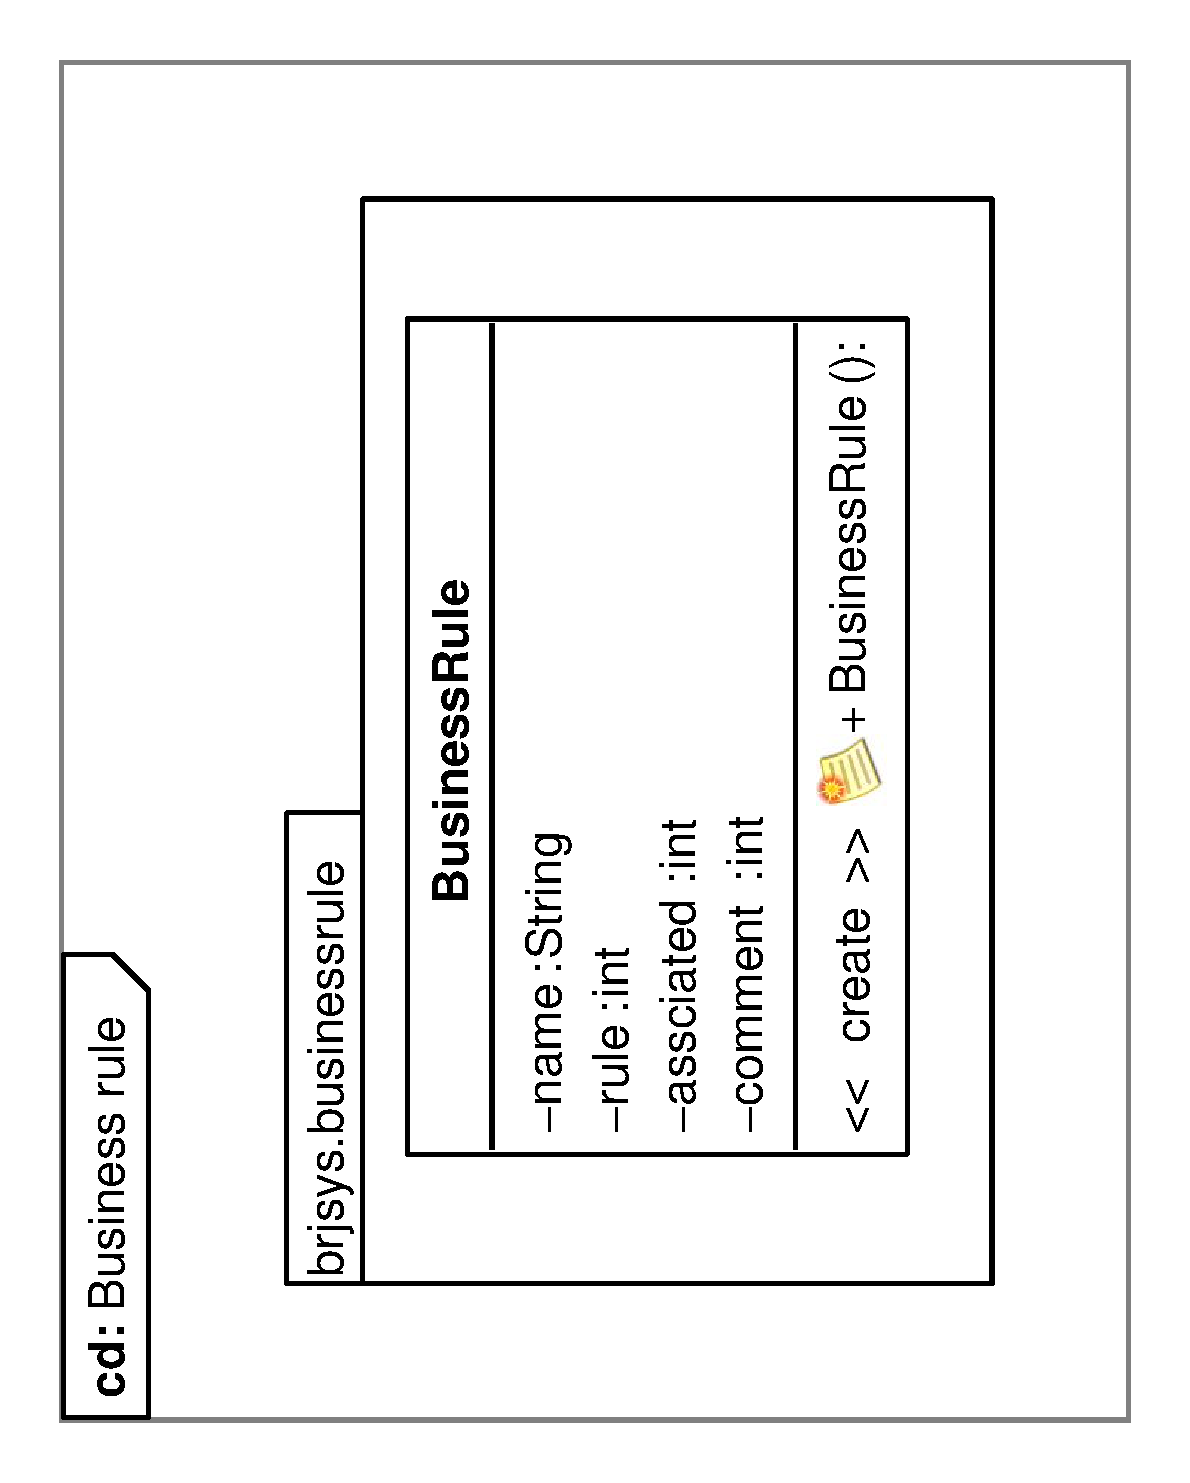
\includegraphics[width=0.3\textwidth, angle=-90]{DiagrammaClassi/Businessrule.eps}
\end{center}
\subsection{BusinessRule}
\subsubsection{Tipo, obiettivo e funzione del componente}
La componente \BR\ rappresenta la \br\ che l'utente inserisce e vuole validare.
\subsubsection{Relazioni d'uso di altre componenti}
Nessuna.
\subsubsection{Interfacce con e relazioni di uso da altre componenti}
La componente GUI utilizza \BR\ nel caso in cui l'utente voglia inserire una nuova \br.
La componente Validator effettua la validazione di un'istanza di \BR, tramite la chiamata del suo metodo validate().
\subsubsection{Attivit\`a svolte e dati trattati}
La componente contiene i campi dato Stringa per rappesentare una business rule (name, associatedObject, rule e comment, dove quest'ultimo pu\`o non essere istanziato). Vengono inoltre messi a disposizione il costruttore e il metodo ridefinito toString().

\section{Comunicatore}
\subsection{Diagramma delle classi}
\begin{center}
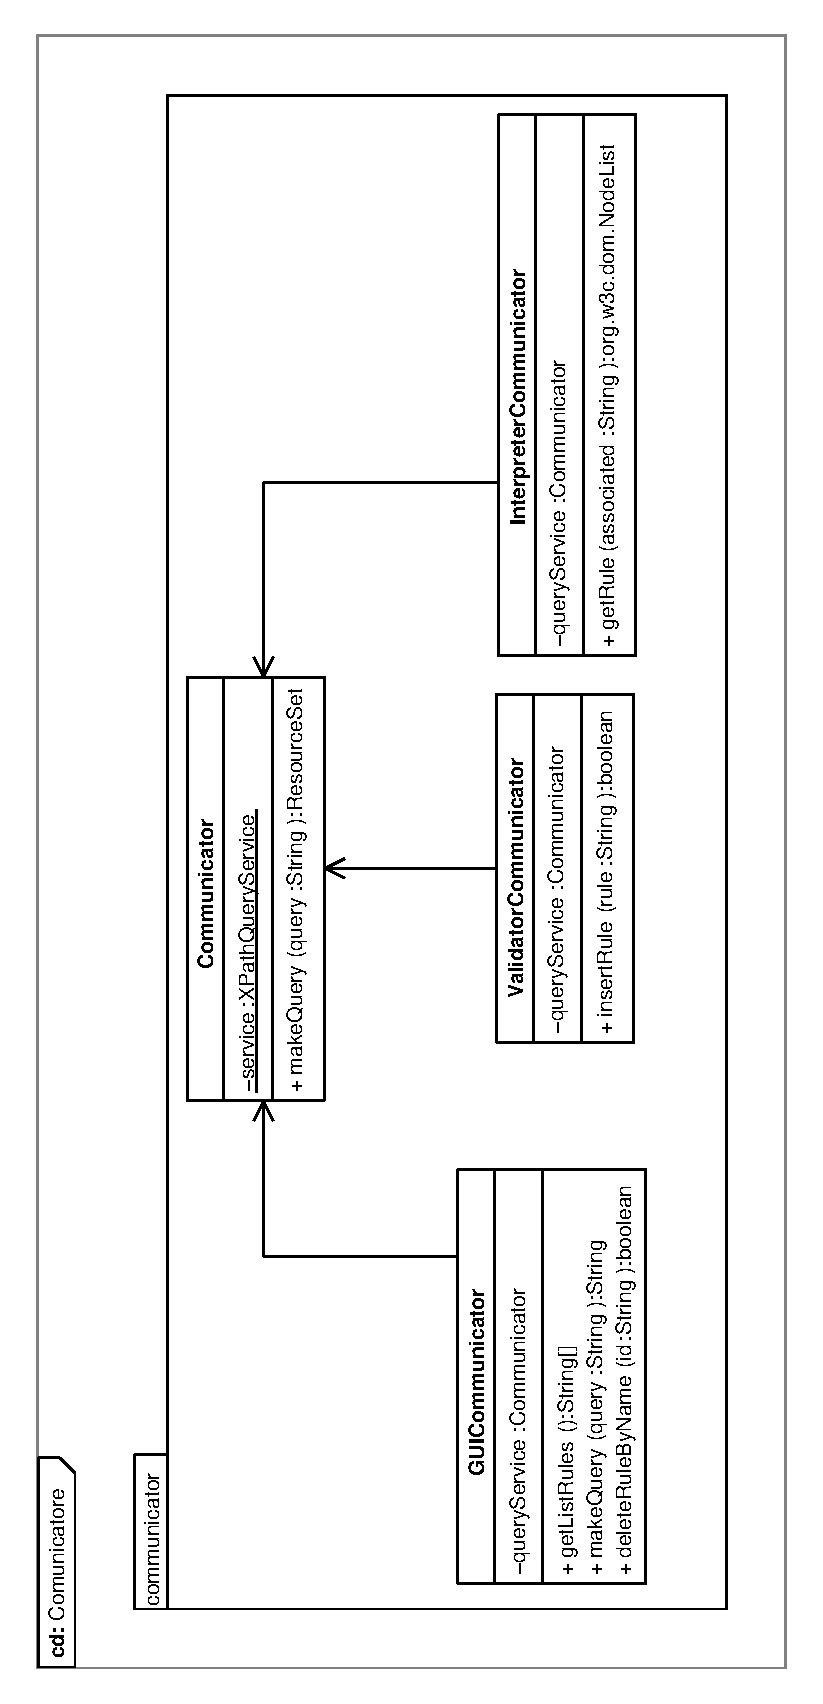
\includegraphics[width=0.5\textwidth, angle=-90]{DiagrammaClassi/Comunicatore.eps}
\end{center}
\subsection{Communicator}
\subsubsection{Tipo, obiettivo e funzione del componente}
Communicator fornisce alle componenti che la utilizzano la possibilit\`a di effettuare query di qualsiasi tipo al \re\ presente nel DBMS.
\subsubsection{Relazioni d'uso di altre componenti}
Communicator necessita di interagire con la componente esterna DBMS per interrogare il \re.
\subsubsection{Interfacce con e relazioni di uso da altre componenti}
Le componenti GUICommunicator, InterpreterCommunicator e ValidatorCommunicator necessitano di Communicator per potergli passare Query specifiche. Le loro descrizioni verranno trattate successivamente.
\subsubsection{Attivit\`a svolte e dati trattati}
Quando viene istanziata per la prima volta, inizializza la connessione al DBMS tramite la definizione di una variabile statica. Successivamente Communicator consente di interrogare il \re\ direttamente, passandogli la stringa che rappresenta la query composta secondo le specifiche XQuery.
%
\subsection{GUICommunicator}
\subsubsection{Tipo, obiettivo e funzione del componente}
La componente contiene metodi necessari per modellare query di cancellazione (tramite operazioni XQuery Update) e query di semplice interrogazione.
\subsubsection{Relazioni d'uso di altre componenti}
GUICommunicator utilizza la componente Communicator per accedere al \re\ ed interrogarlo.
\subsubsection{Interfacce con e relazioni di uso da altre componenti}
GUICommunicator viene messa in relazione con la componente GUI, dalla quale riceve richieste di cancellazione e di querying.
\subsubsection{Attivit\`a svolte e dati trattati}
GUICommunicator fornisce le operazioni:
\begin{itemize}
 \item deleteRuleByName(): dato il nome di una regola, provvede ad eliminarla dal \re\ nel caso questa regola sia presente;
 \item makeQuery(): permette l'esecuzione di una semplice query purch\`e non implichi modifiche strutturali al \re;
 \item getListRules(): ritorna per ogni \br, nome, \bo\ associato e struttura.
\end{itemize}
\subsection{InterpreterCommunicator}
\subsubsection{Tipo, obiettivo e funzione del componente}
InterpreterCommunicator contiene metodi necessari per rispondere a richieste di \br\ da parte di un interprete esterno.
\subsubsection{Relazioni d'uso di altre componenti}
InterpreterCommunicator utilizza la componente Communicator per accedere al \re\ ed interrogarlo.
\subsubsection{Interfacce con e relazioni di uso da altre componenti}
La componente InterpreterCommunicator viene messa in relazione con l'interprete esterno, dal quale riceve richieste di \brs associate ad un determinato \bo.
\subsubsection{Attivit\`a svolte e dati trattati}
InterpreterCommunicator offre il metodo getRule() per richiedere le \br\ associate al \bo.

\subsection{ValidatorCommunicator}
\subsubsection{Tipo, obiettivo e funzione del componente}
ValidatorCommunicator contiene metodi necessari per effettuare l'inserimento di una \br\ validata gi\`a tradotta in XML.
\subsubsection{Relazioni d'uso di altre componenti}
ValidatorCommunicator utilizza la componente Communicator per accedere al \re\ ed interrogarlo.
\subsubsection{Interfacce con e relazioni di uso da altre componenti}
ValidatorCommunicator viene messa in relazione con la componente Validator per effettuare l'inserimento.
\subsubsection{Attivit\`a svolte e dati trattati}
ValidatorCommunicator offre il metodo insertRule() per inserire la \br\ nel \re. L'inserimento avverr\`a soltanto se la \br\ ha un nome che non \`e ancora presente nel \re.

\chapter{Componenti esterne}
\begin{center}
 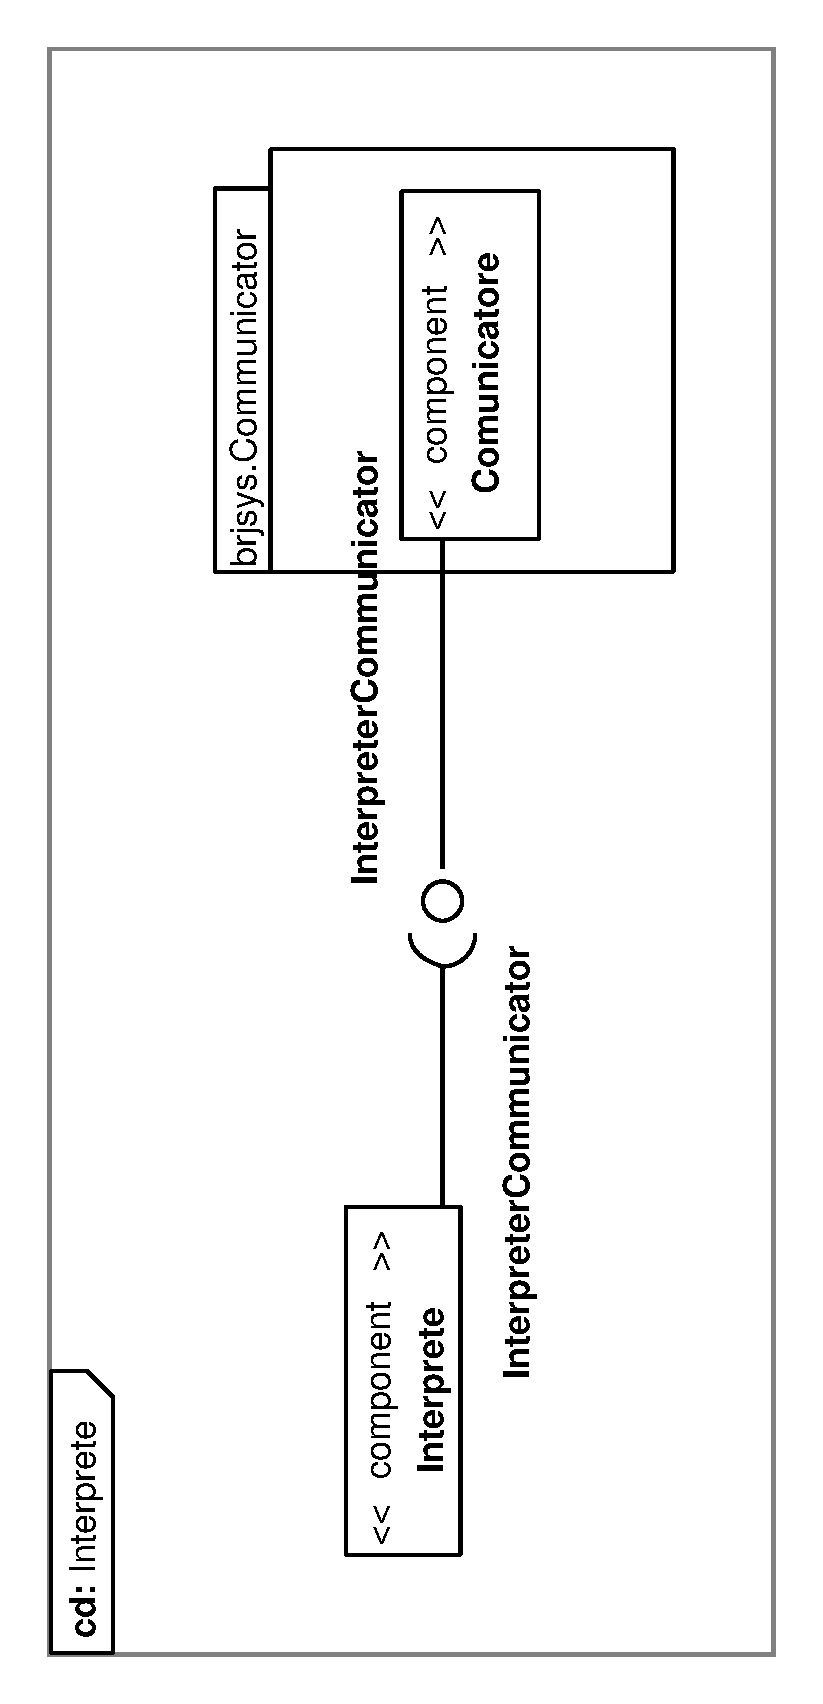
\includegraphics[width=0.5\textwidth, angle=-90]{DiagrammaClassi/Interprete.eps}
\end{center}
\section{Interprete}
\subsubsection{Tipo, obiettivo e funzione del componente}
Questo componente si incarica di eseguire le \brs\ associate ad un determinato \bo. Per ottenere le \brs\ il componente deve poter interrogare il DBMS attraverso un opportuna interfaccia col sistema BR-jsys che risolver\`a per lui la richiesta.
\subsubsection{Relazioni d'uso di altre componenti}
Interprete utilizza la componente InterpreterCommunicator per comunicare col DBMS.
\subsubsection{Interfacce con e relazioni di uso da altre componenti}
Nessuna.
\subsubsection{Attivit\`a svolte e dati trattati}
Non siamo tenuti a considerare i dettagli riguardanti le operazioni specifiche della componente. L'unico vincolo posto \`e che comunichi con il DBMS tramite l'interfaccia InterpreterCommunicator.
\section{DBMS}
\begin{center}
 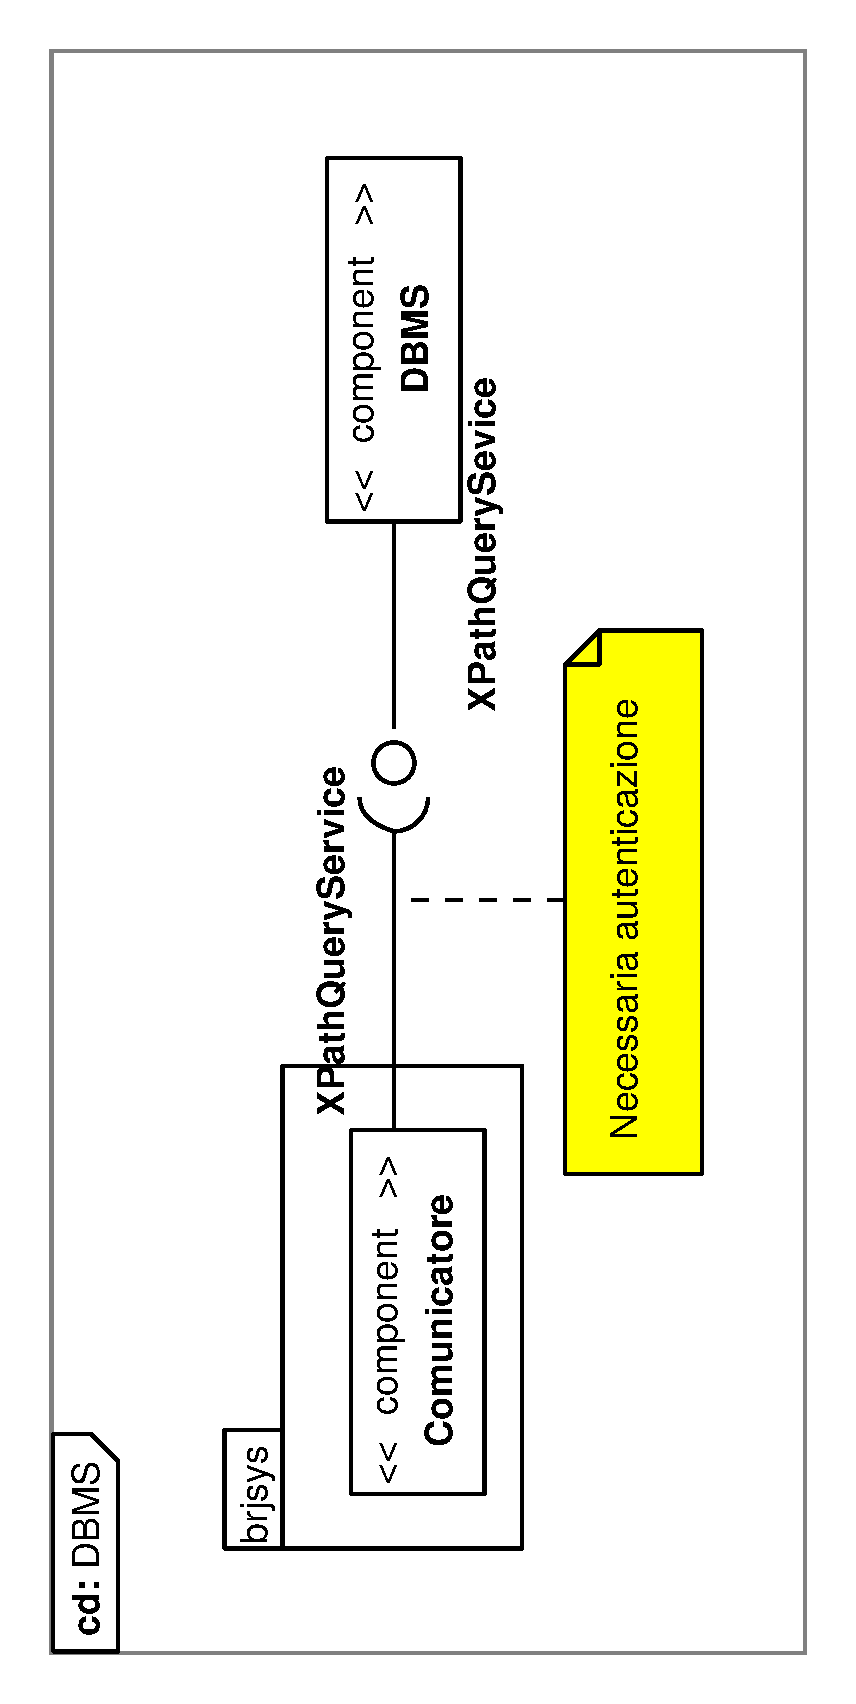
\includegraphics[width=0.5\textwidth, angle=-90]{DiagrammaClassi/DBMS.eps}
\end{center}
\subsubsection{Tipo, obiettivo e funzione del componente}
Questa componente serve a comunicare con il \re\ in modo efficiente. La comunicazione avverr\`a tramite linguaggio XQuery.
\subsubsection{Relazioni d'uso di altre componenti}
Nessuna.
\subsubsection{Interfacce con e relazioni di uso da altre componenti}
Previa una connessione corretta, il DBMS mette a disposizione un'interfaccia XPathQueryService con la quale interagire col \re\ presente all'interno del DBMS stesso.
\subsubsection{Attivit\`a svolte e dati trattati}
Una corretta autenticazione far\`a in modo che l'interfaccia di tipo XPathQueryService possa interagire col \re tramite il metodo query(). Quest'ultimo accetta come parametro una query impostata secondo le specifiche XQuery.


\chapter{Diagrammi di attivit\`a}


\section{Server DBMS}
\begin{center}
 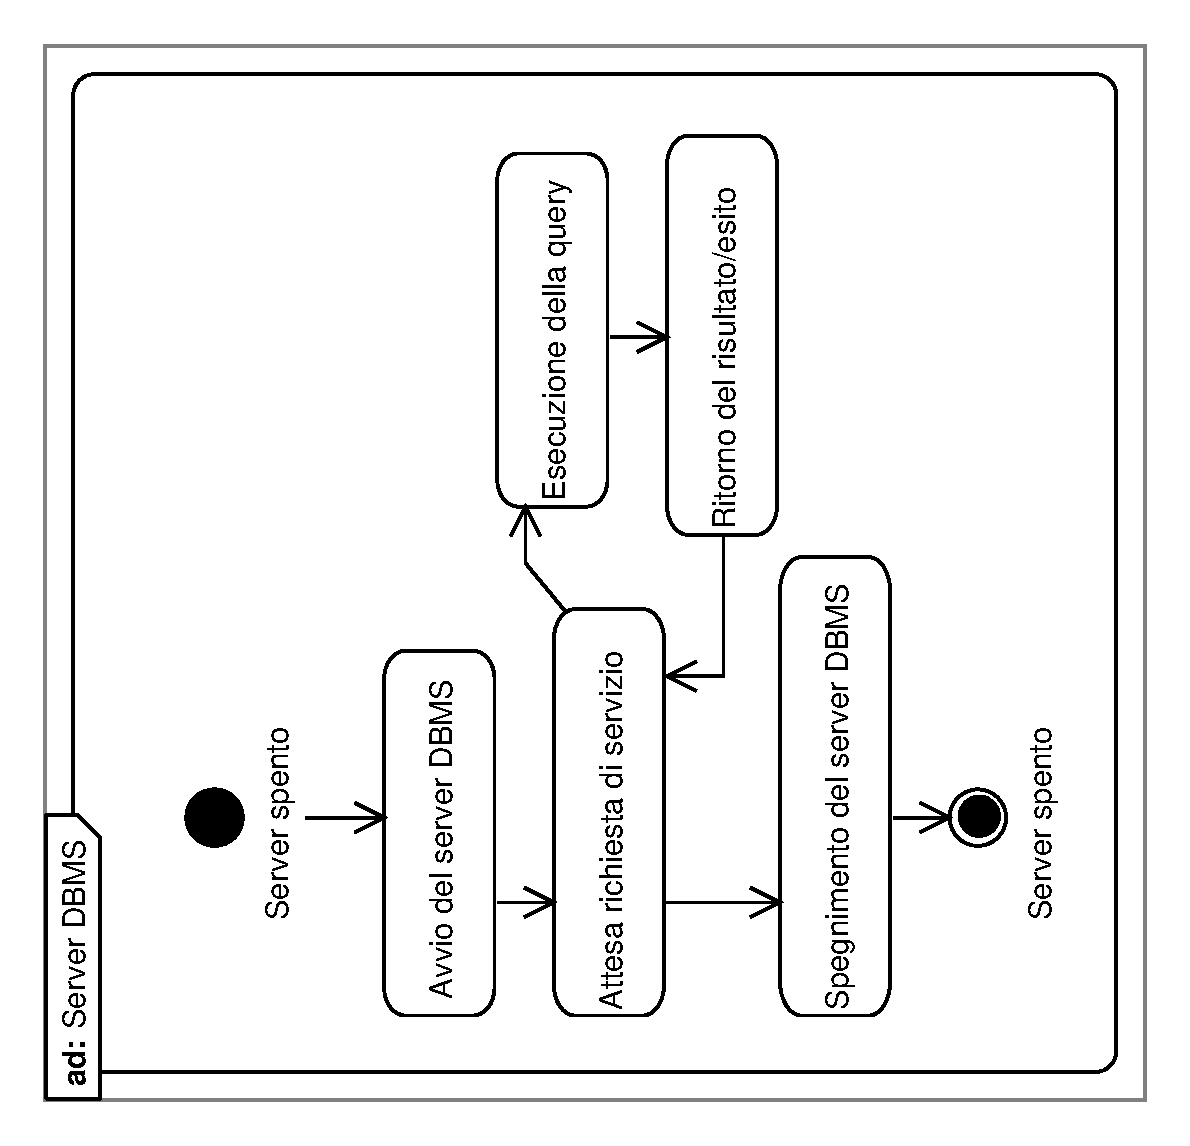
\includegraphics[width=0.5\textwidth, angle=-90]{Server.eps}
\end{center}
Il server DBMS, con il quale interagisce il prodotto ``BR-jsys'', viene avviato. Una volta completata la procedura di avvio entra in uno stato di attesa di richieste da parte della GUI e dell'interprete. Ricevuta una richiesta, la relativa query viene inviata al DBMS e il risultato/esito della query viene ritornato all'utente. Il server torna quindi in uno stato di attesa, finch\`e eventualmente viene spento.

\section{Richiesta dell'interprete}
\begin{center}
 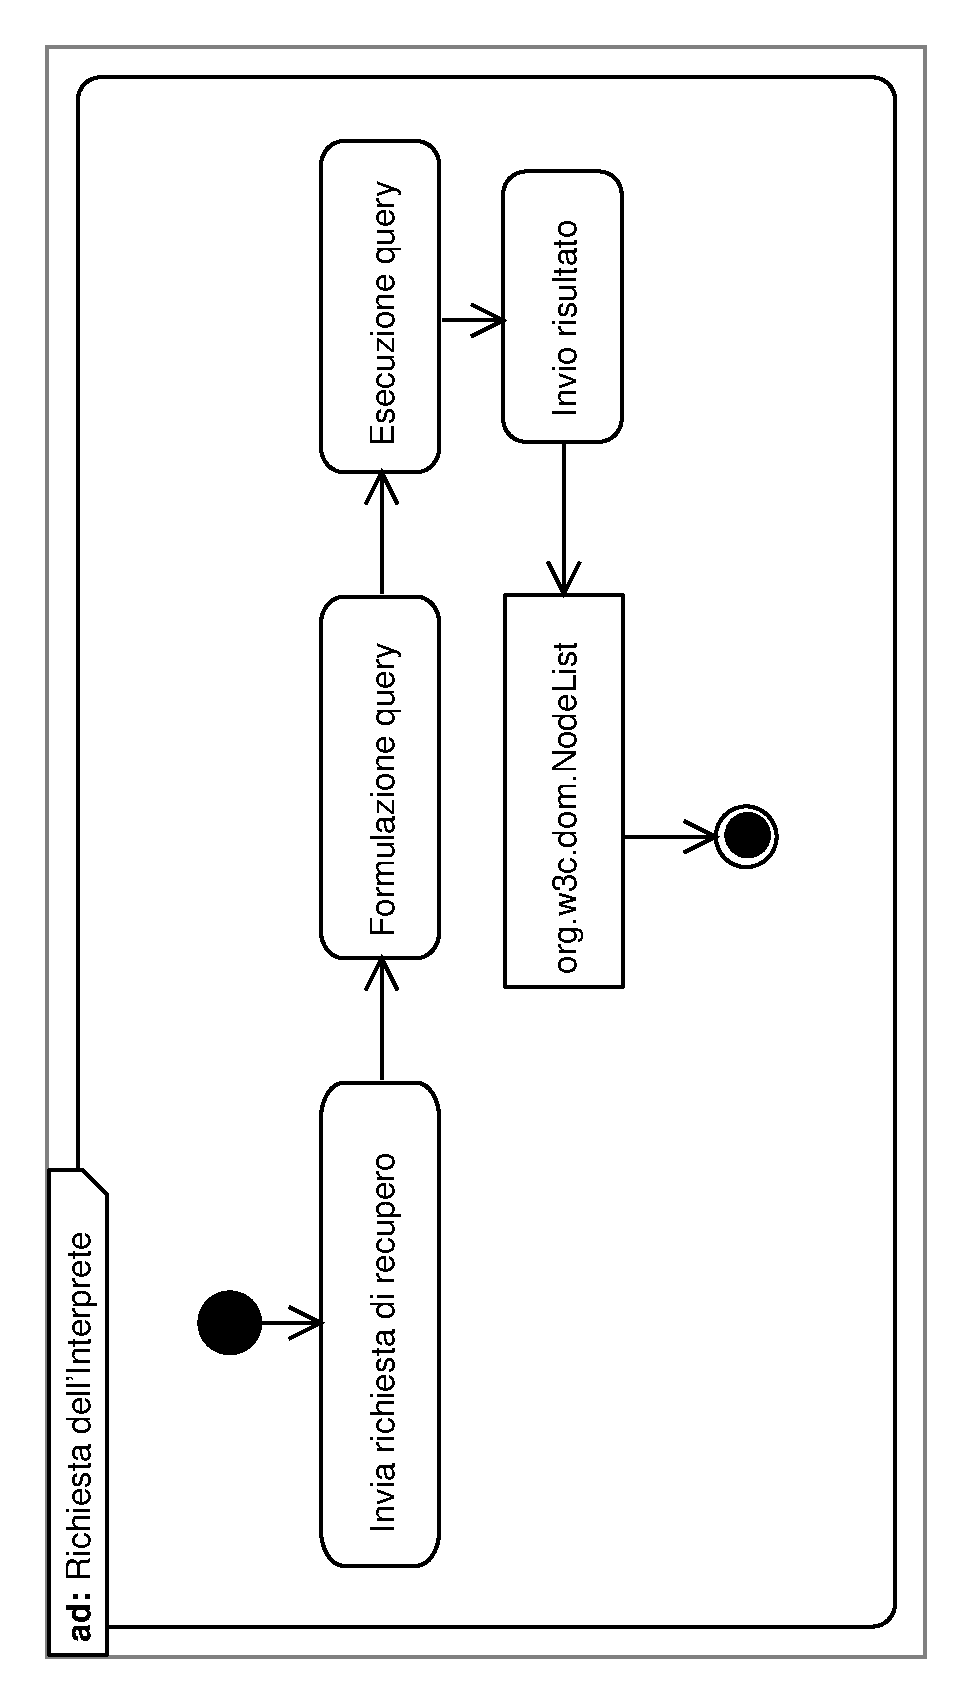
\includegraphics[width=0.5\textwidth, angle=-90]{RichiestadellInterprete.eps}
\end{center}
L'interprete invia la richiesta al sistema, il quale formula la query da inviare al DBMS. La query viene quindi eseguita e il risultato viene tornato all'interprete sottoforma di un oggetto \textit{org.w3c.dom.NodeList}.

\section{GUI}
\begin{center}
 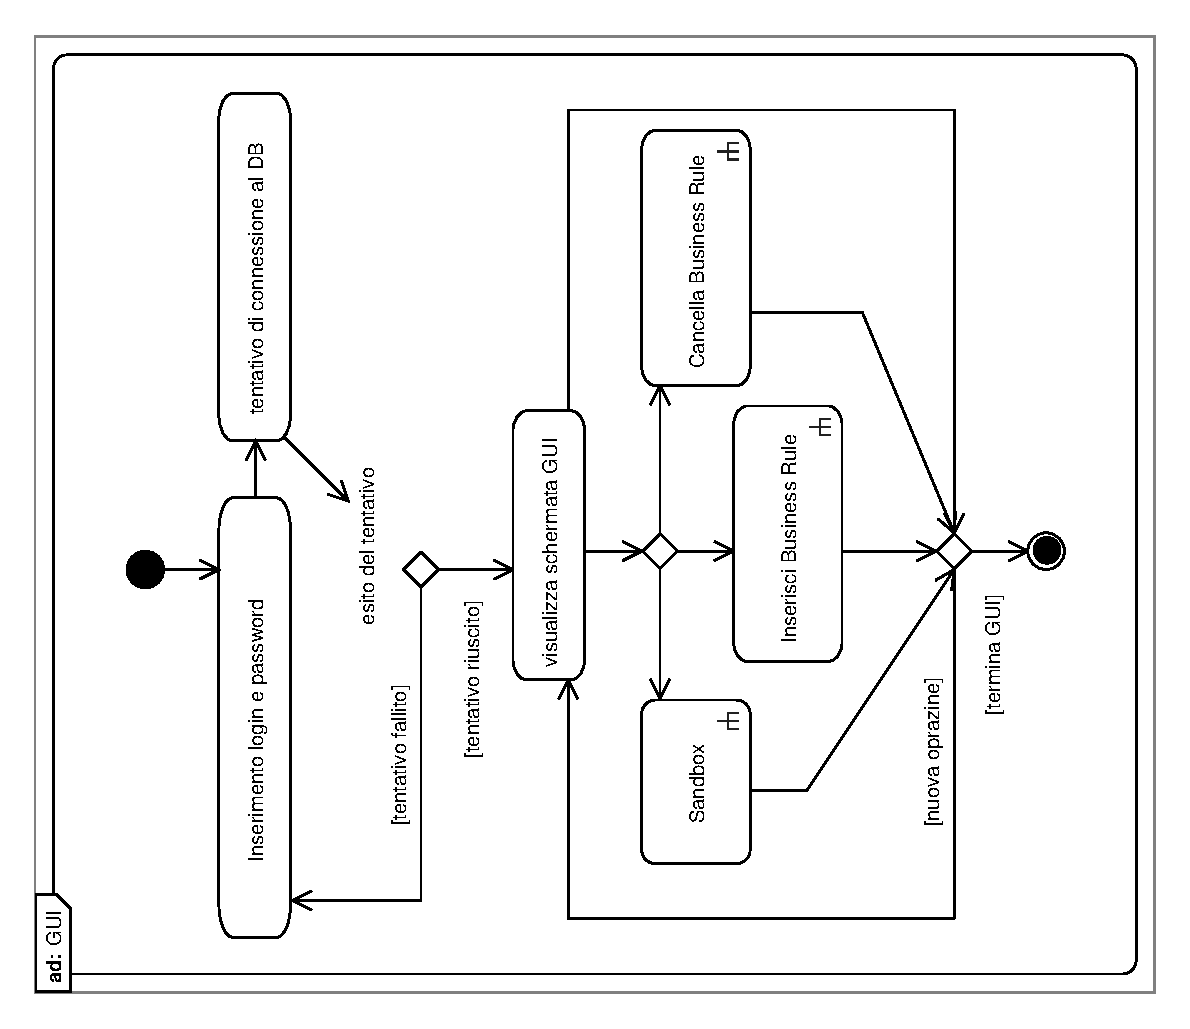
\includegraphics[width=1\textwidth, angle=-90]{GUI.eps}
\end{center}
All'avvio della GUI viene visualizzato un messaggio in cui vengono richiesti \textit{login} e \textit{password}. Si cerca quindi di stabilire una connessione qualificata al DB. 
Si controlla quindi l'esito del tentativo di connessione; se il tentativo ha dato esito negativo si richiede la \textit{login} e la
 \textit{password} all'utente. Se, al contrario, l'esito e positivo, ossia si ha disposizione una connessione, viene visualizzata la schermata della GUI dalla quale
 possono essere lanciati :\textit{ l'inserimento di una \br} , \textit{l'avvio di una Sandbox}, \textit{la cancellazione di una \br}.
Nel diagramma queste tre attvit\`a sono rappresentate come delle \textit{sub-activity} che vengono illustrate di seguito. Al termine di ogni operazione l'utente viene riportato alla finestra principale dove pu\`o effettuare una nuova operazione oppure terminare l'esecuzione della GUI stessa.

\section{Inserisci \br}
\begin{center}
 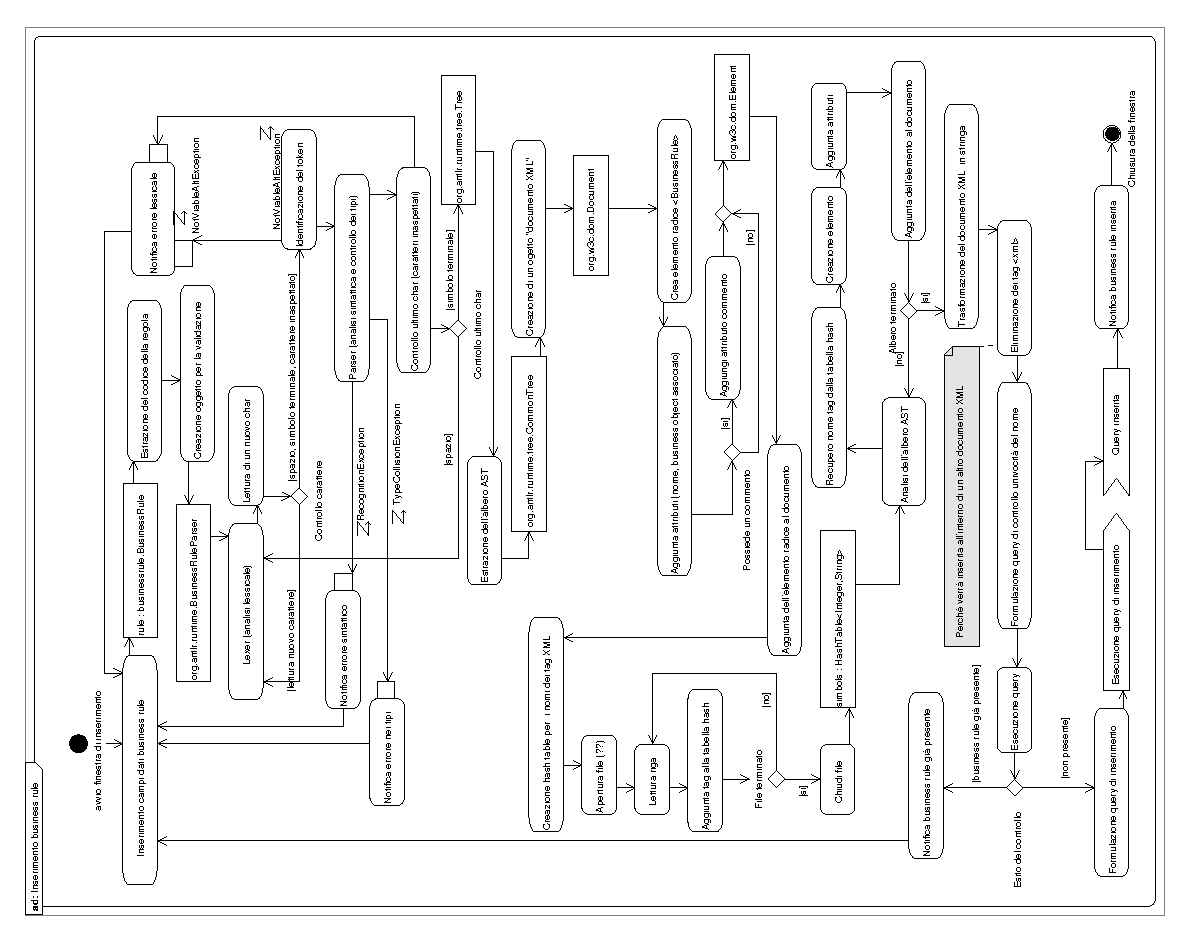
\includegraphics[width=1.4\textwidth, angle=-90]{InserisciBusinessRule2.eps}
\end{center}


\section{Sandbox}
\begin{center}
 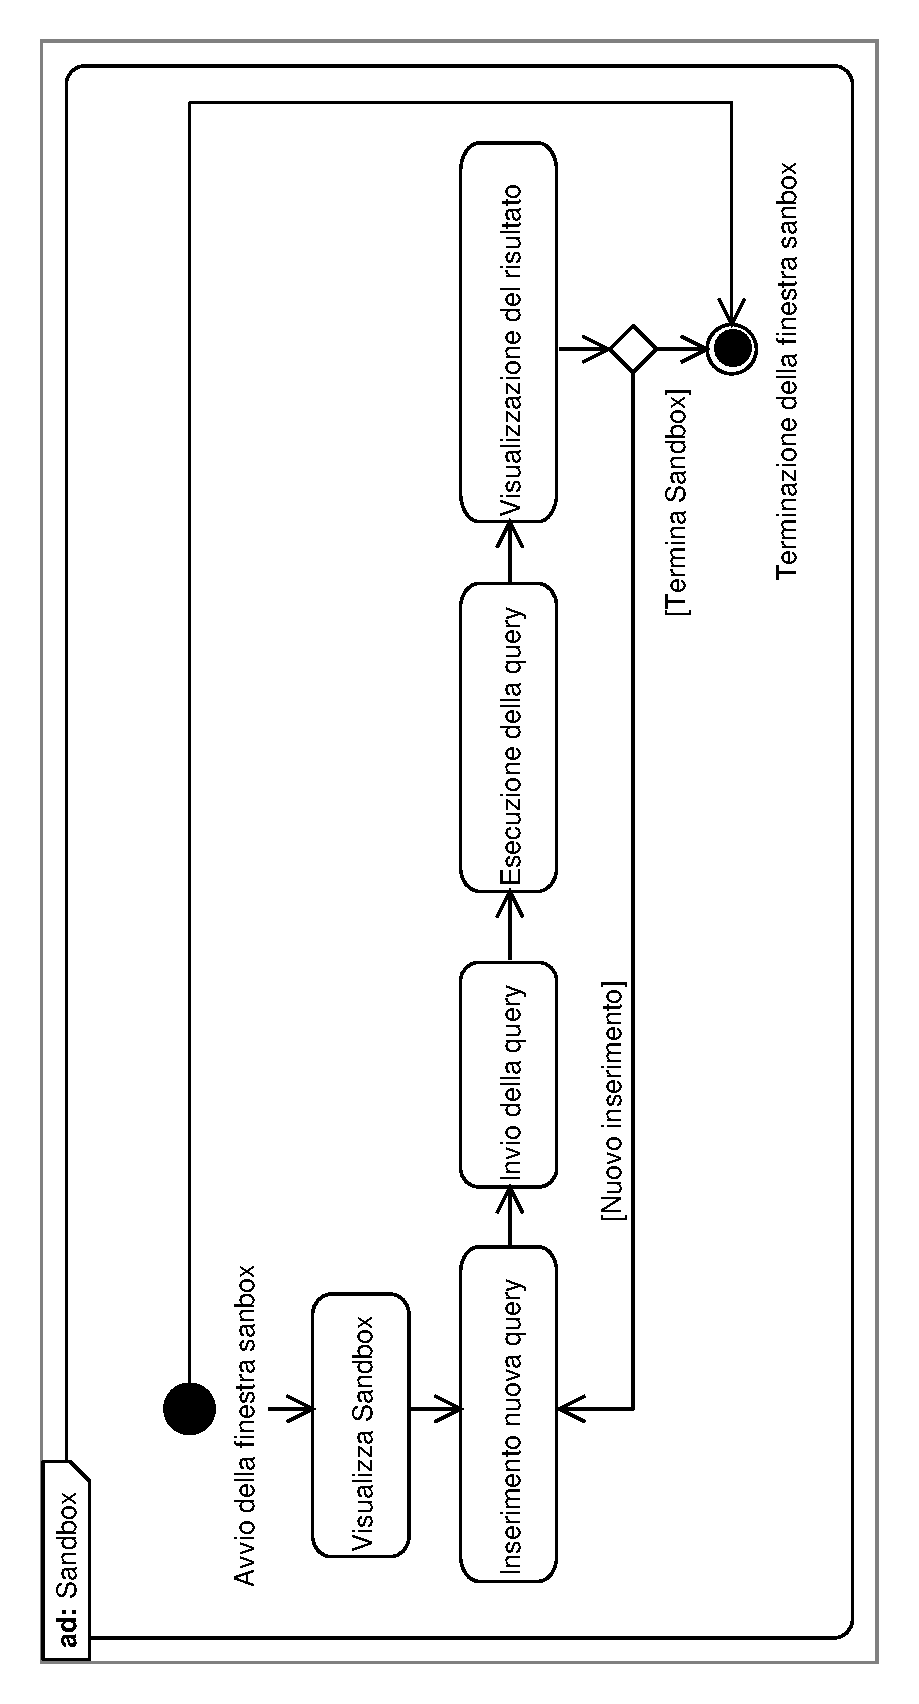
\includegraphics[width=0.5\textwidth, angle=-90]{Sandbox.eps}
\end{center}
La \textit{Sandbox} \`e una finestra il cui scopo \`e permettere ad un utente di eseguire dei test sul repository. Viene quindi fornito uno spazio in cui digitare una query. La query viene inviata al DBMS ed eseguita. Vengono infine presentati a video i risultati della query evidenziando il tempo impiegato per ottenerli. L'utente pu\`o poi terminare la finestra \textit{Sandbox} o inserire una nuova query.

\section{Cancellazione \br}
\begin{center}
 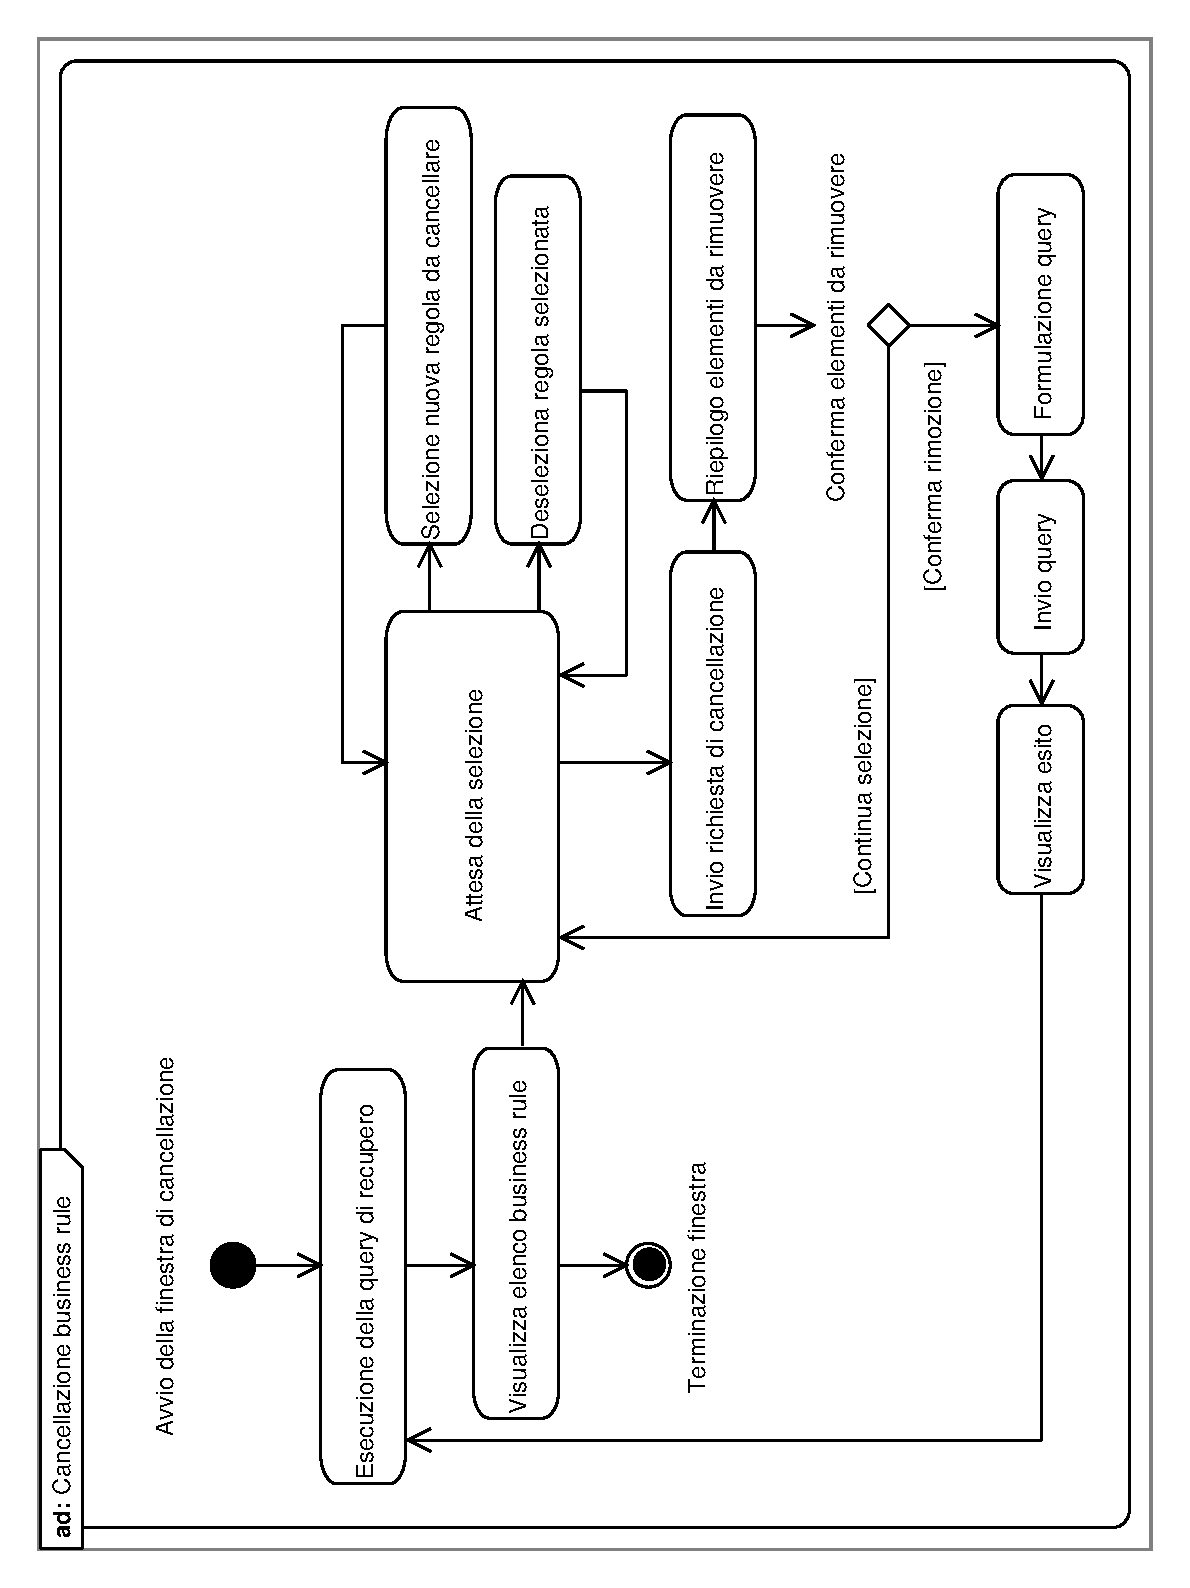
\includegraphics[width=0.7\textwidth, angle=-90]{CancellazioneBusinessRule.eps}
\end{center}
Viene inizialmente effettuata una query sul DBMS atta a recuperare un elenco completo delle \brs. Una volta recuperato l'elenco delle \brs\ presenti nel \re\ queste vengono visualizzate sinteticamente in forma tabellare, accompagnate da una \textit{checkbox}. Si attende quindi la selezione/deselezione dell'utente. L'utente notifica al sistema (mediante un bottone) l'intenzione di cancellare le \brs\ selezionate.  Viene poi mostrato un riepilogo delle \brs che verranno eliminate. Se l'utente non conferma il sistema torna ad attendere la selezione. Se invece la rimozione viene confermata, allora si formula la query di rimozione, la quale viene infine eseguita. Al termine della rimozione viene effettuata nuovamente una query di recupero per visualizzare le \brs\ rimaste nel \re.


%\chapter{Diagrammi di sequenza}
%\chapter{Diagrammi di collaborazione}

\chapter{Stime di fattibilit\`a e di bisogno di risorse}
Dopo aver analizzato il problema attraverso schemi progettuali sono state individuate le risorse necessarie per la realizzazione del prodotto. Con l'utilizzo di software open source siamo riusciti a contenere i costi e contemporaneamente a rendere disponibili tutte le risorse.
Tutte queste risorse necessarie ai nostri componenti per affrontare le varie problematiche di comunicazione, lo sviluppo del codice, la gestione degli archivi, la verifica dei documenti e del sistema, sono state descritte nel documento \PdQ.
Nella fase di specifica tecnica e successivamente di progettazione verranno utilizzati diagrammi UML realizzati con \textit{Poseidon for UML Professional edition 6.0.2} nella versione trial in quanto pi\`u completo e usabile rispetto ad altri software simili come ad esempio ArgoUML. Solo i diagrammi use case sono stati realizzati con Dia in quanto progettati prima di affidarsi a Poseidon.
Il progetto sar\`a realizzato mediante il linguaggio java come da requisito implicito del capitolato. Useremo la versione 6 essendo quella di pi\`u recente sviluppo.
Per la produzione della Gui e delle classi java abbiamo utilizzato Eclipse versione 3.3.1.1, un IDE in grado di fornire numerose funzionalit\`a per lo sviluppo del software.
Per la parte riguardante la grammatica, dopo varie ricerche e confronti, ci siamo affidati invece ad Antlr 3.0.1 come generatore di parser e AntlrWorks 1.1.5 come ambiente grafico di sviluppo in quanto offrivano la maggior chiarezza e risposta alle nostre aspettative.
Tutta la documentazione sar\`a redatta utilizzando Kile 2.0 un user-friendly Tex/Latex editor completo e chiaro nelle sue funzionalit\`a.
Lo sviluppo avr\`a luogo singolarmente o in piccoli gruppi a seconda della natura della problematica da affrontare.
Il documento/codice avr\`a ad ogni modo un unico proprietario incaricato di renderlo pubblico tramite server SVN.
Utilizzando queste risorse e visti i tempi di consegna del prodotto, la ditta HappyCodeInc ritiene quindi soddisfacibili le richieste del committente.
Per tempistiche pi\`u dettagliate si rimanda al \PdP.

\chapter{Tracciamento della relazione componenti-requisiti}

\begin{center}
\begin{table}[hbtp]
\large{
\begin{tabular}{l}
\begin{tabular}{||p{3cm}||p{5cm}||p{6cm}||} \hline \hline
\textbf{Componente} & \textbf{Componente Specifico} & \textbf{Requisiti Associati} \\ \hline

GUI & & F4, F5, F7, F8\\ \hline
 &  & \\ \hline

Validatore & Validator & F2, F3, F4, F5, F8, NPR1, NQ1\\ \hline
 & BusinessRuleLexer & F2, F4, NQ1 \\ \hline
 & BusinessRuleParser & F2, F4, F10, NQ1 \\ \hline
 & TypeCollisionException & F2, F4, F10, NQ1\\ \hline
 & XMLParser & NPo1\\ \hline
 & businessobjects & F2, F10, F11\\ \hline
 &  & \\ \hline

BusinessRule & & F2, F10, F11, NU1, NU2, NU3, NQ1\\ \hline
 &  & \\ \hline

Comunicatore & Communicator & F3, F5, F6, NPr1\\ \hline
 & GUICommunicator & F5, F7, F8\\ \hline
 & InterpreterCommunicator & F5, F6\\ \hline
 & ValidatorCommunicator & F3\\ \hline


\end{tabular} \\
\end{tabular}

}
\end{table}
\end{center}




\end{document}

    
